\chapter{Prova de conceito}
\label{cha:prova-de-conceito}

	Para o fornecimento e consumo de serviços entre Componentes I4.0 Clientes (C4.0-Cliente) e Componentes I4.0 Servidores (C4.0-Servidor), diversos protocolos e tecnologias podem ser adotadas.
	
	Este capítulo tem o objetivo de apresentar uma implementação funcional da arquitetura apresentada no \autoref{cha:arquitetura} como prova de conceito, adotando alguns protocolos e tecnologias comumente utilizadas em engenharia de \textit{software} e desenvolvimento de sistemas.
	

\section{Arquitetura do WS e tecnologias utilizadas}

	O protocolo de comunicação para o fornecimento de WSs mais comumente aplicado atualmente é o HTTP \cite{gruner2016restful}, seguindo as regras de operações padronizadas definidas pelo padrão REST.
	
	Alguns outros protocolos também são aplicados para oferecimentos de WSs, como o MQTT, que está presente principalmente na área de automação residencial e IoT \cite{yokotani2016mqtt}.


\section{Estruturação dos dados da MDP}

	A estrutura proposta usa o padrão de troca de dados JSON, que utiliza texto legível a humanos, no formato atributo-valor (natureza auto-descritiva). O formato de intercâmbio de informações no formato JSON é usado em WSs que usam transferência de estado representacional (REST) e aplicações AJAX, substituindo o uso do XML.
	
	A estrutura de armazenamento implementada usa banco de dados orientado a documentos que usa documento em formato JSON com esquemas pré-definidos.
	
	A \autoref{fig:json} mostra um exemplo de estruturação de dados para troca e armazenamento de informações em JSON.
	
	\begin{figure}[htb]
		\centering
		\caption{Formato de intercâmbio de informações da MDP em JSON.}
		\label{fig:json}
		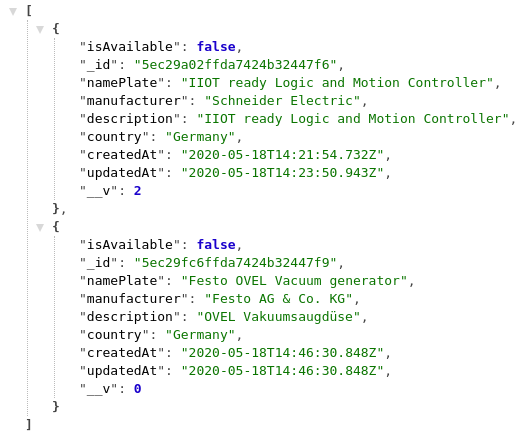
\includegraphics[width=0.8\textwidth]{json}
		\fonte{O autor.}
	\end{figure}

	
\section{API de interação Cliente-Servidor}

	A interação entre Cliente e Servidor é realizada por meio de API REST.
	
	A API REST é invocada como uma interface para acesso aos serviços de um C4.0-Servidor, podendo extrair dados internos de sua MDP e executar operações CRUD (criação, leitura, atualização e exclusão).
	